\documentclass{standalone}
\usepackage{tikz}
\usetikzlibrary{patterns, positioning}

\begin{document}
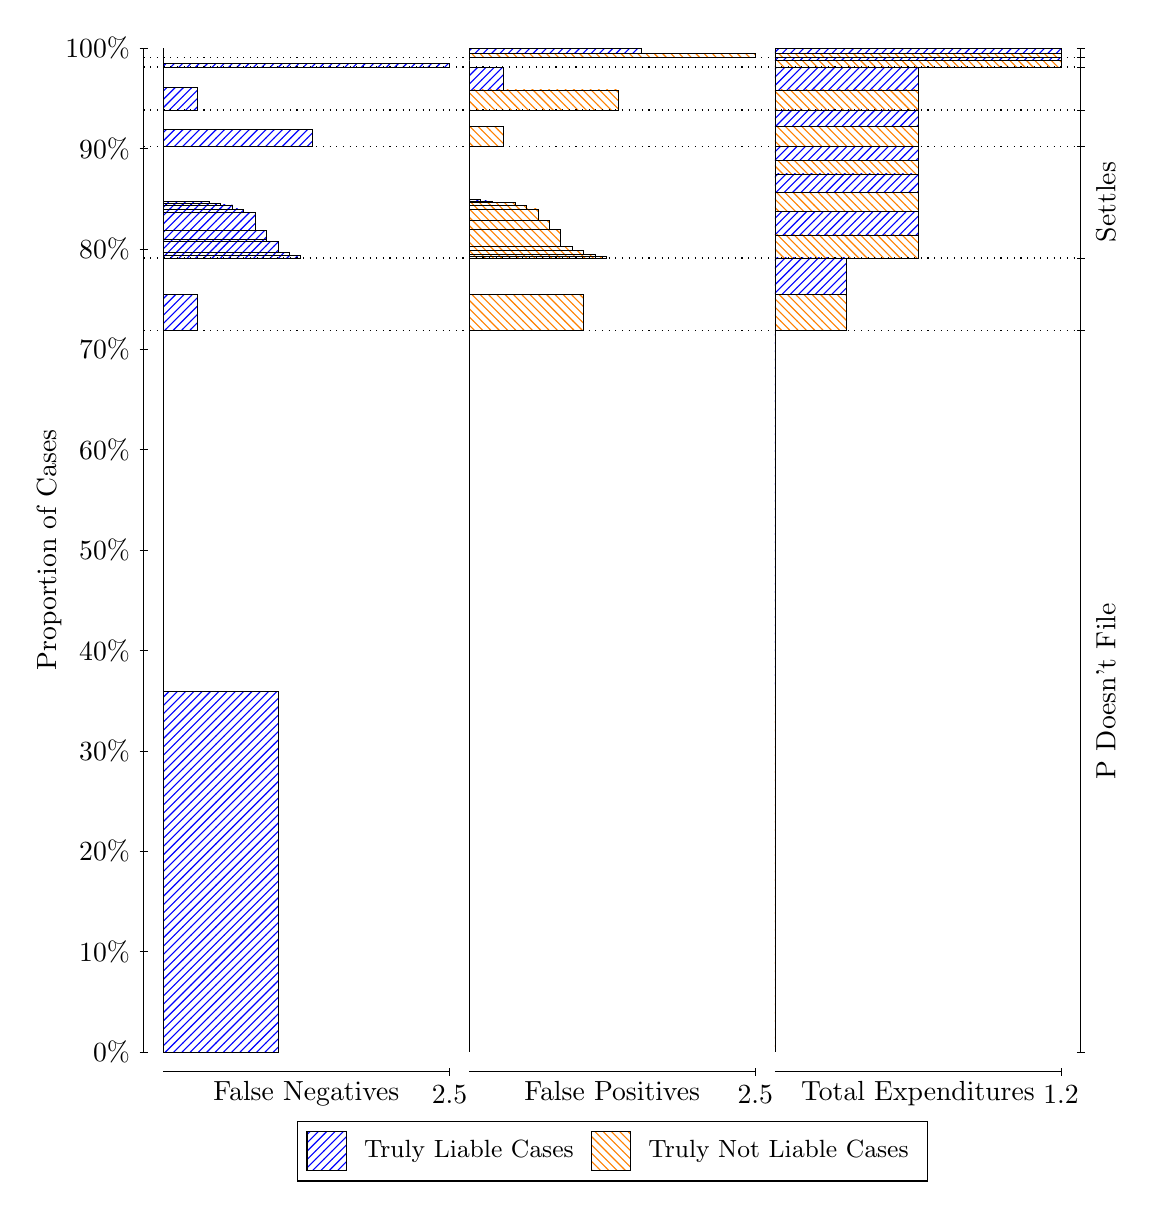
\begin{tikzpicture}
\draw[black, very thin] (1.5,1.75) -- (1.5,14.5);
\node[rotate=90, anchor=center] at (0.3, 8.125) {Proportion of Cases};
\draw[black, very thin] (1.45,1.75) -- (1.55,1.75);
\node[anchor=east] at (1.45, 1.75) {0\%};
\draw[black, very thin] (1.45,3.025) -- (1.55,3.025);
\node[anchor=east] at (1.45, 3.025) {10\%};
\draw[black, very thin] (1.45,4.3) -- (1.55,4.3);
\node[anchor=east] at (1.45, 4.3) {20\%};
\draw[black, very thin] (1.45,5.575) -- (1.55,5.575);
\node[anchor=east] at (1.45, 5.575) {30\%};
\draw[black, very thin] (1.45,6.85) -- (1.55,6.85);
\node[anchor=east] at (1.45, 6.85) {40\%};
\draw[black, very thin] (1.45,8.125) -- (1.55,8.125);
\node[anchor=east] at (1.45, 8.125) {50\%};
\draw[black, very thin] (1.45,9.4) -- (1.55,9.4);
\node[anchor=east] at (1.45, 9.4) {60\%};
\draw[black, very thin] (1.45,10.675) -- (1.55,10.675);
\node[anchor=east] at (1.45, 10.675) {70\%};
\draw[black, very thin] (1.45,11.95) -- (1.55,11.95);
\node[anchor=east] at (1.45, 11.95) {80\%};
\draw[black, very thin] (1.45,13.225) -- (1.55,13.225);
\node[anchor=east] at (1.45, 13.225) {90\%};
\draw[black, very thin] (1.45,14.5) -- (1.55,14.5);
\node[anchor=east] at (1.45, 14.5) {100\%};

\draw[black, very thin] (13.4,1.75) -- (13.4,14.5);
\draw[black, very thin] (13.35,1.75) -- (13.45,1.75);
\node[anchor=west] at (13.35, 1.75) {};
\draw[black, very thin] (13.35,10.914) -- (13.45,10.914);
\node[anchor=west] at (13.35, 10.914) {};
\draw[black, very thin] (13.35,11.834) -- (13.45,11.834);
\node[anchor=west] at (13.35, 11.834) {};
\draw[black, very thin] (13.35,13.253) -- (13.45,13.253);
\node[anchor=west] at (13.35, 13.253) {};
\draw[black, very thin] (13.35,13.713) -- (13.45,13.713);
\node[anchor=west] at (13.35, 13.713) {};
\draw[black, very thin] (13.35,14.259) -- (13.45,14.259);
\node[anchor=west] at (13.35, 14.259) {};
\draw[black, very thin] (13.35,14.383) -- (13.45,14.383);
\node[anchor=west] at (13.35, 14.383) {};
\draw[black, very thin] (13.35,14.5) -- (13.45,14.5);
\node[anchor=west] at (13.35, 14.5) {};

\draw[black, very thin, pattern color=blue, pattern=north east lines] (1.75,1.75) rectangle (3.2033,6.3319);
\draw[black, very thin, pattern color=orange, pattern=north west lines] (1.75,6.3319) rectangle (1.75,10.914);
\draw[black, very thin, pattern color=blue, pattern=north east lines] (1.75,10.914) rectangle (2.186,11.374);
\draw[black, very thin, pattern color=orange, pattern=north west lines] (1.75,11.374) rectangle (1.75,11.834);
\draw[black, very thin, pattern color=blue, pattern=north east lines] (1.75,11.834) rectangle (3.494,11.869);
\draw[black, very thin, pattern color=blue, pattern=north east lines] (1.75,11.869) rectangle (3.3487,11.902);
\draw[black, very thin, pattern color=blue, pattern=north east lines] (1.75,11.902) rectangle (3.2033,12.049);
\draw[black, very thin, pattern color=blue, pattern=north east lines] (1.75,12.049) rectangle (3.058,12.066);
\draw[black, very thin, pattern color=blue, pattern=north east lines] (1.75,12.066) rectangle (3.058,12.18);
\draw[black, very thin, pattern color=blue, pattern=north east lines] (1.75,12.18) rectangle (2.9127,12.412);
\draw[black, very thin, pattern color=blue, pattern=north east lines] (1.75,12.412) rectangle (2.7673,12.458);
\draw[black, very thin, pattern color=blue, pattern=north east lines] (1.75,12.458) rectangle (2.622,12.508);
\draw[black, very thin, pattern color=blue, pattern=north east lines] (1.75,12.508) rectangle (2.4767,12.529);
\draw[black, very thin, pattern color=blue, pattern=north east lines] (1.75,12.529) rectangle (2.3313,12.55);
\draw[black, very thin, pattern color=orange, pattern=north west lines] (1.75,12.55) rectangle (1.75,13.253);
\draw[black, very thin, pattern color=blue, pattern=north east lines] (1.75,13.253) rectangle (3.6393,13.466);
\draw[black, very thin, pattern color=orange, pattern=north west lines] (1.75,13.466) rectangle (1.75,13.713);
\draw[black, very thin, pattern color=blue, pattern=north east lines] (1.75,13.713) rectangle (2.186,14.003);
\draw[black, very thin, pattern color=orange, pattern=north west lines] (1.75,14.003) rectangle (1.75,14.259);
\draw[black, very thin, pattern color=blue, pattern=north east lines] (1.75,14.259) rectangle (5.3833,14.301);
\draw[black, very thin, pattern color=orange, pattern=north west lines] (1.75,14.301) rectangle (1.75,14.383);
\draw[black, very thin, pattern color=orange, pattern=north west lines] (1.75,14.383) rectangle (1.75,14.427);
\draw[black, very thin, pattern color=blue, pattern=north east lines] (1.75,14.427) rectangle (1.75,14.5);
\draw[black, very thin, pattern color=orange, pattern=north west lines] (5.6333,1.75) rectangle (5.6333,6.3319);
\draw[black, very thin, pattern color=blue, pattern=north east lines] (5.6333,6.3319) rectangle (5.6333,10.914);
\draw[black, very thin, pattern color=orange, pattern=north west lines] (5.6333,10.914) rectangle (7.0867,11.374);
\draw[black, very thin, pattern color=blue, pattern=north east lines] (5.6333,11.374) rectangle (5.6333,11.834);
\draw[black, very thin, pattern color=orange, pattern=north west lines] (5.6333,11.834) rectangle (7.3773,11.855);
\draw[black, very thin, pattern color=orange, pattern=north west lines] (5.6333,11.855) rectangle (7.232,11.875);
\draw[black, very thin, pattern color=orange, pattern=north west lines] (5.6333,11.875) rectangle (7.0867,11.929);
\draw[black, very thin, pattern color=orange, pattern=north west lines] (5.6333,11.929) rectangle (6.9413,11.98);
\draw[black, very thin, pattern color=orange, pattern=north west lines] (5.6333,11.98) rectangle (6.796,12.198);
\draw[black, very thin, pattern color=orange, pattern=north west lines] (5.6333,12.198) rectangle (6.6507,12.314);
\draw[black, very thin, pattern color=orange, pattern=north west lines] (5.6333,12.314) rectangle (6.5053,12.456);
\draw[black, very thin, pattern color=orange, pattern=north west lines] (5.6333,12.456) rectangle (6.36,12.5);
\draw[black, very thin, pattern color=orange, pattern=north west lines] (5.6333,12.5) rectangle (6.2147,12.537);
\draw[black, very thin, pattern color=blue, pattern=north east lines] (5.6333,12.537) rectangle (5.924,12.558);
\draw[black, very thin, pattern color=blue, pattern=north east lines] (5.6333,12.558) rectangle (5.7787,12.579);
\draw[black, very thin, pattern color=blue, pattern=north east lines] (5.6333,12.579) rectangle (5.6333,13.253);
\draw[black, very thin, pattern color=orange, pattern=north west lines] (5.6333,13.253) rectangle (6.0693,13.5);
\draw[black, very thin, pattern color=blue, pattern=north east lines] (5.6333,13.5) rectangle (5.6333,13.713);
\draw[black, very thin, pattern color=orange, pattern=north west lines] (5.6333,13.713) rectangle (7.5227,13.968);
\draw[black, very thin, pattern color=blue, pattern=north east lines] (5.6333,13.968) rectangle (6.0693,14.259);
\draw[black, very thin, pattern color=orange, pattern=north west lines] (5.6333,14.259) rectangle (5.6333,14.341);
\draw[black, very thin, pattern color=blue, pattern=north east lines] (5.6333,14.341) rectangle (5.6333,14.383);
\draw[black, very thin, pattern color=orange, pattern=north west lines] (5.6333,14.383) rectangle (9.2667,14.427);
\draw[black, very thin, pattern color=blue, pattern=north east lines] (5.6333,14.427) rectangle (7.8133,14.5);
\draw[black, very thin, pattern color=orange, pattern=north west lines] (9.5167,1.75) rectangle (9.5167,6.3319);
\draw[black, very thin, pattern color=blue, pattern=north east lines] (9.5167,6.3319) rectangle (9.5167,10.914);
\draw[black, very thin, pattern color=orange, pattern=north west lines] (9.5167,10.914) rectangle (10.425,11.374);
\draw[black, very thin, pattern color=blue, pattern=north east lines] (9.5167,11.374) rectangle (10.425,11.834);
\draw[black, very thin, pattern color=orange, pattern=north west lines] (9.5167,11.834) rectangle (11.333,12.126);
\draw[black, very thin, pattern color=blue, pattern=north east lines] (9.5167,12.126) rectangle (11.333,12.428);
\draw[black, very thin, pattern color=orange, pattern=north west lines] (9.5167,12.428) rectangle (11.333,12.669);
\draw[black, very thin, pattern color=blue, pattern=north east lines] (9.5167,12.669) rectangle (11.333,12.901);
\draw[black, very thin, pattern color=orange, pattern=north west lines] (9.5167,12.901) rectangle (11.333,13.072);
\draw[black, very thin, pattern color=blue, pattern=north east lines] (9.5167,13.072) rectangle (11.333,13.253);
\draw[black, very thin, pattern color=orange, pattern=north west lines] (9.5167,13.253) rectangle (11.333,13.5);
\draw[black, very thin, pattern color=blue, pattern=north east lines] (9.5167,13.5) rectangle (11.333,13.713);
\draw[black, very thin, pattern color=orange, pattern=north west lines] (9.5167,13.713) rectangle (11.333,13.968);
\draw[black, very thin, pattern color=blue, pattern=north east lines] (9.5167,13.968) rectangle (11.333,14.259);
\draw[black, very thin, pattern color=orange, pattern=north west lines] (9.5167,14.259) rectangle (13.15,14.341);
\draw[black, very thin, pattern color=blue, pattern=north east lines] (9.5167,14.341) rectangle (13.15,14.383);
\draw[black, very thin, pattern color=orange, pattern=north west lines] (9.5167,14.383) rectangle (13.15,14.427);
\draw[black, very thin, pattern color=blue, pattern=north east lines] (9.5167,14.427) rectangle (13.15,14.5);
\draw[black, dotted] (1.5,10.914) -- (13.4,10.914);
\draw[black, dotted] (1.5,11.834) -- (13.4,11.834);
\draw[black, dotted] (1.5,13.253) -- (13.4,13.253);
\draw[black, dotted] (1.5,13.713) -- (13.4,13.713);
\draw[black, dotted] (1.5,14.259) -- (13.4,14.259);
\draw[black, dotted] (1.5,14.383) -- (13.4,14.383);
\draw[black, very thin] (1.75,1.5) -- (5.3833,1.5);
\node[anchor=north] at (3.5667, 1.5) {False Negatives};
\draw[black, very thin] (5.3833,1.45) -- (5.3833,1.55);
\node[anchor=north] at (5.3833, 1.45) {2.5};

\draw[black, very thin] (5.6333,1.5) -- (9.2667,1.5);
\node[anchor=north] at (7.45, 1.5) {False Positives};
\draw[black, very thin] (9.2667,1.45) -- (9.2667,1.55);
\node[anchor=north] at (9.2667, 1.45) {2.5};

\draw[black, very thin] (9.5167,1.5) -- (13.15,1.5);
\node[anchor=north] at (11.333, 1.5) {Total Expenditures};
\draw[black, very thin] (13.15,1.45) -- (13.15,1.55);
\node[anchor=north] at (13.15, 1.45) {1.2};

\node[black, centered, rotate=90] at (13.72, 6.3319) {P Doesn't File};

\node[black, centered, rotate=90] at (13.72, 12.544) {Settles};





\draw (7.449999999999999,1.5) node[draw=none] (baseCoordinate) {};
\begin{scope}[align=center]
        \matrix[scale=0.5, draw=black, below=0.5cm of baseCoordinate, nodes={draw}, column sep=0.1cm]{
            \node[rectangle, draw, minimum width=0.5cm, minimum height=0.5cm, pattern=north east lines, pattern color=blue] {}; &
            \node[draw=none, font=\small] (B) {Truly Liable Cases}; &
            \node[rectangle, draw, minimum width=0.5cm, minimum height=0.5cm, pattern=north west lines, pattern color=orange] {}; &
            \node[draw=none, font=\small] (B) {Truly Not Liable Cases}; \\
            };
\end{scope}

\end{tikzpicture}
\end{document}